\item \points{15} {\bf Kernelizing the Perceptron}

Let there be a binary classification problem with $y \in \{0, 1\}$.  The
perceptron uses hypotheses of the form $h_\theta(x) = g(\theta^T x)$, where
$g(z) = \text{sign}(z) = 1$ if $z \ge 0$, $0$ otherwise.  In this problem we
will consider a stochastic gradient descent-like implementation of the
perceptron algorithm where each update to the parameters $\theta$ is made using
only one training example.  However, unlike stochastic gradient descent, the
perceptron algorithm will only make one pass through the entire training set.
The update rule for this version of the perceptron algorithm is given by
\begin{equation*}
  \theta^{(i+1)} :=
	  \theta^{(i)} + \alpha (y^{(i+1)} - h_{\theta^{(i)}}(x^{(i+1)})) x^{(i+1)}
\end{equation*}
where $\theta^{(i)}$ is the value of the parameters after the algorithm has
seen the first $i$ training examples. Prior to seeing any training examples,
$\theta^{(0)}$ is initialized to $\vec{0}$.

\begin{enumerate}
  \item \subquestionpoints{9} Let $K$ be a Mercer kernel corresponding to some
very high-dimensional feature
mapping $\phi$. Suppose $\phi$ is so high-dimensional (say,
$\infty$-dimensional) that it's infeasible to ever represent $\phi(x)$
explicitly.  Describe how you would apply the ``kernel trick'' to the
perceptron to make it work in the high-dimensional feature space $\phi$, but
without ever explicitly computing $\phi(x)$.

[\textbf{Note:} You don't have to worry about the intercept term.  If you like,
think of $\phi$ as having the property that $\phi_0(x) = 1$ so that this is
taken care of.] Your description should specify:
\begin{enumerate}[label=\roman*.]
  \item \subquestionpoints{3} How you will (implicitly) represent the
  high-dimensional
    parameter vector $\theta^{(i)}$, including how the initial value
    $\theta^{(0)} = 0$ is represented (note that $\theta^{(i)}$ is
    now a vector whose dimension is the same as the feature vectors
    $\phi(x)$);
  \item \subquestionpoints{3} How you will efficiently make a prediction on a
  new input
    $x^{(i+1)}$.  I.e., how you will compute
    $h_{\theta^{(i)}}(x^{(i+1)}) = g({\theta^{(i)}}^T \phi(x^{(i+1)}))$,
    using your representation of $\theta^{(i)}$; and
  \item \subquestionpoints{3} How you will modify the update rule given above
  to perform an
  update to $\theta$ on a new training example $(x^{(i+1)}, y^{(i+1)})$;
  \emph{i.e.,} using the update rule corresponding to the feature mapping
  $\phi$:
  \begin{equation*}
  \theta^{(i+1)} :=
	  \theta^{(i)} + \alpha (y^{(i+1)} - h_{\theta^{(i)}}(x^{(i+1)})) x^{(i+1)}
  \end{equation*}
\end{enumerate}

\ifnum\solutions=1 {
  \begin{answer}
\end{answer}

} \fi


\ifnum\solutions=1 {
  \begin{answer}
\end{answer}

} \fi

  \item \subquestionpoints{5} Implement your approach by completing the
\texttt{initial\_state}, \texttt{predict}, and \texttt{update\_state} methods
of \texttt{src/p05\_percept.py}.


\ifnum\solutions=1 {
  \begin{answer}

\begin{figure}[htbp]
    \centering
    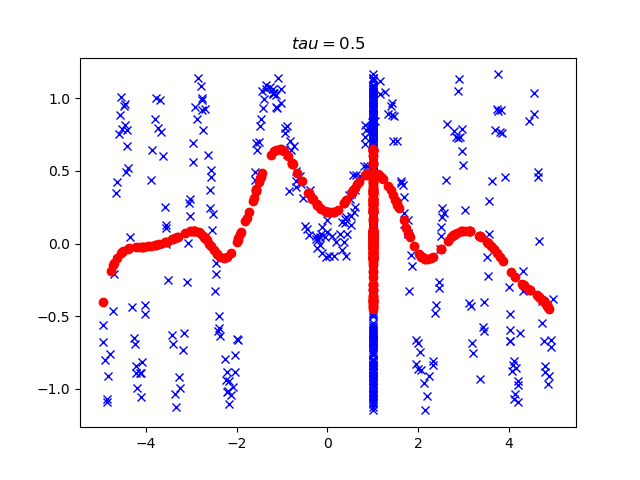
\includegraphics[width=0.5\linewidth]{pics/tau_0d5.png}
    \caption{tau=0.5}
\end{figure}

Final MSE is $0.33$. The model seems to underfitting.

\end{answer}

} \fi


  \item \subquestionpoints{2} 
One of the choices in Q4b completely fails, one works a bit, and one works well in classifying the points.
Discuss the performance of different choices and why do they fail or perform well?



\ifnum\solutions=1 {
  \begin{answer}
\end{answer}

} \fi

\end{enumerate}
